Эксперименты ставились на парах искусственных изображений и на реально отснятых оптических изображениях

\subsection{Искусственные изображения}

В качестве образцов брались несколько видов текстур приведены на рисунках ниже.

\begin{figure}[ht]
\center{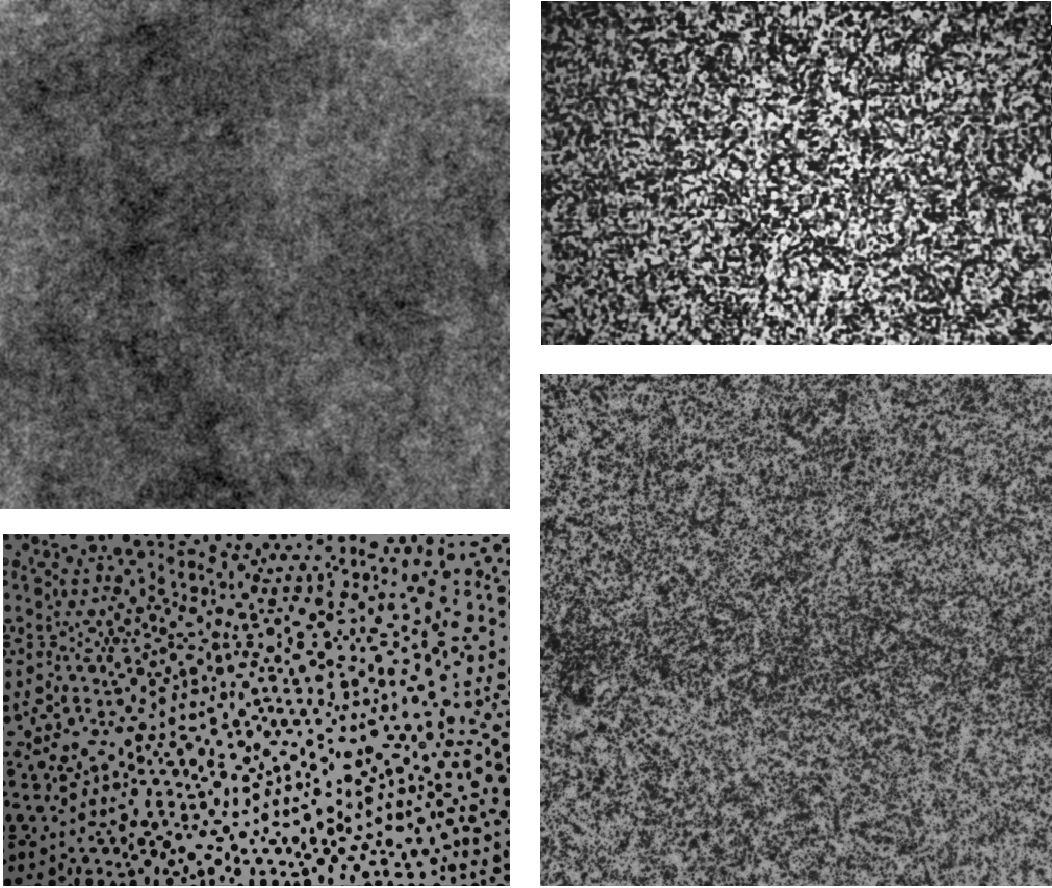
\includegraphics[width=0.8\linewidth]{gray_mix}}
\caption{Тестовая серия изображений: По часовой стрелке Серая подборка, Тестовая серия №11, Серия высокого контраста, Тестовая серия №6}
\label{pic:gray_mix}
\end{figure}

\subsection{Реальные изображения}

Серия оптических изображений использованных для тестирования программного обеспечения предоставлена Институт физики прочности и материаловедения СО РАН. На серии снимков изображено одноосное растяжение полимерной пластины.

\begin{figure}[ht]
\center{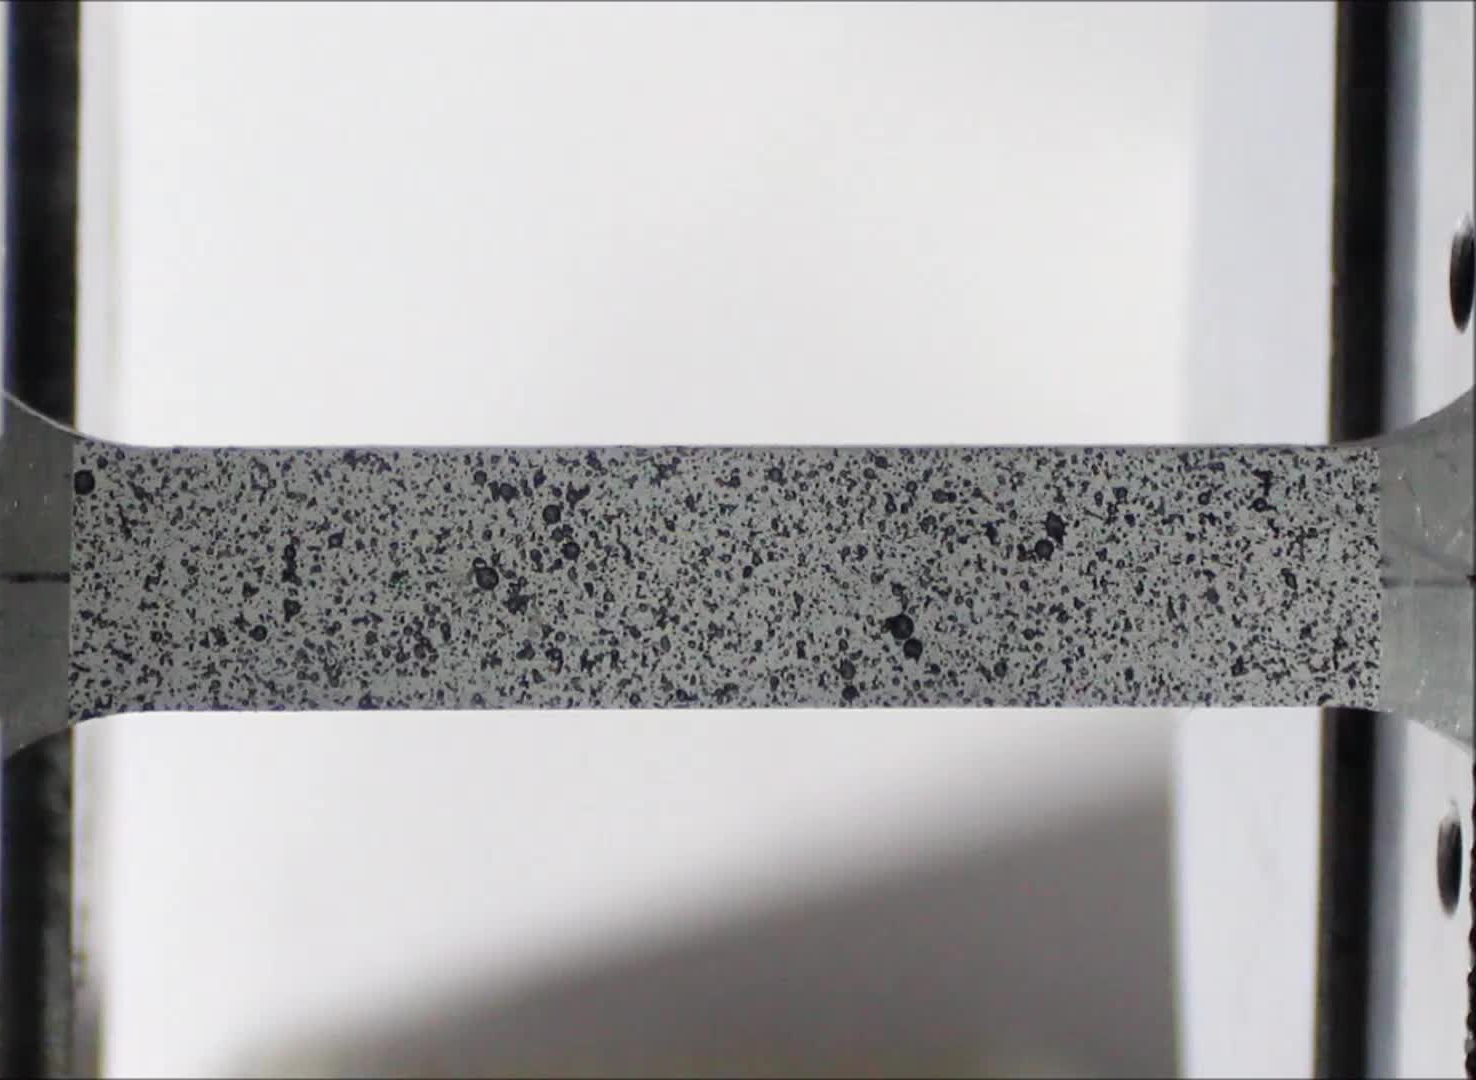
\includegraphics[width=0.6\linewidth]{real_deform}}
\caption{Растяжение полимерной пластины}
\label{pic:real_deform}
\end{figure}
